%%%%%%%%%%%%%%%%%%%%%%%%%%%%%%%%%%%%%%%%%%%%%%%%
% chapter3.tex                                 %
% Contains formatting and content of chapter 3 %
%%%%%%%%%%%%%%%%%%%%%%%%%%%%%%%%%%%%%%%%%%%%%%%%
\chapter{Modeling the Marth-Fox Matchup}
\newpage

\section{Model 1: A Simple Binomial-Beta Conjugate}
For the first model, we will approach it completely analytically. We will model the win rate of a character in a matchup, without factoring in stage choice. Let $\theta$ represent the probability of a character winning a given matchup. Let the likelihood of our model be represented as a binomial distribution $x_i|\theta\sim Bin(n,\theta)$, where $n$ represents the number of matches in the sample. A win for the character would be recorded as a 1 (success), while the loss would be recorded as a 0 (failure). We can specify a Beta prior generally as $\theta\sim Be(\alpha,\beta)$. A Beta prior is flexible, as it allows us to experiment with different initial beliefs for a given matchup.

\indent The Beta prior can form a conjugate distribution with the posterior with respect to the Binomial likelihood. This enables us to find a fully closed-form posterior. Using existing conjugacy tables \citep{brani_vidakovic_2017} p. 341. This gives the posterior $\theta|X\sim Be(\alpha+x, \beta+n-x)$. The mean of the posterior, $\frac{\alpha+x}{(\alpha+x)+(\beta+n-x)}$, gives us the expected win rate for a character in a given matchup.

\indent For the Marth-Fox matchup, assume that we are modeling Marth's win rate against Fox. Below are graphs representing the posterior matchup distribution, given different priors.
% Blah blah blah.  Here is an example of how to include and cite a figure: see Figure~\ref{fig:example_figure}
\begin{figure}[H]
\center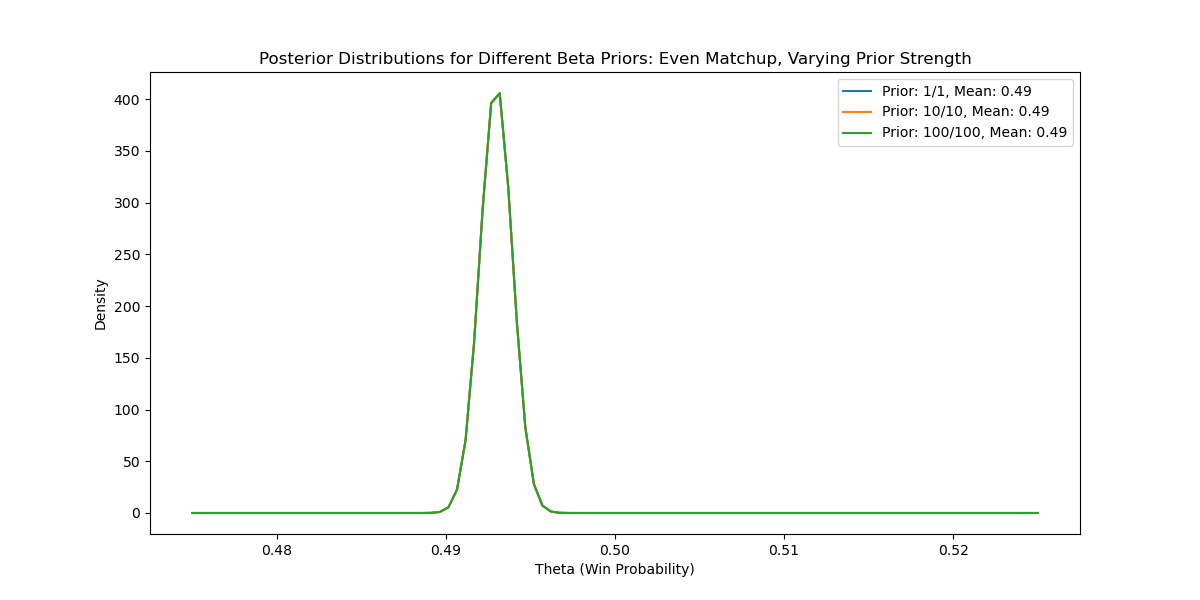
\includegraphics[width=0.8\textwidth]{figures/posterior_beta_priors_varying_strength.png}
\caption[Modeling a 50/50 Marth-Fox matchup prior with varying strengths.]{Modeling a Marth-Fox even (50/50) matchup prior with varying strengths.}
\label{fig:posterior_beta_priors_varying_strength}
\end{figure}
\begin{figure}[H]
\center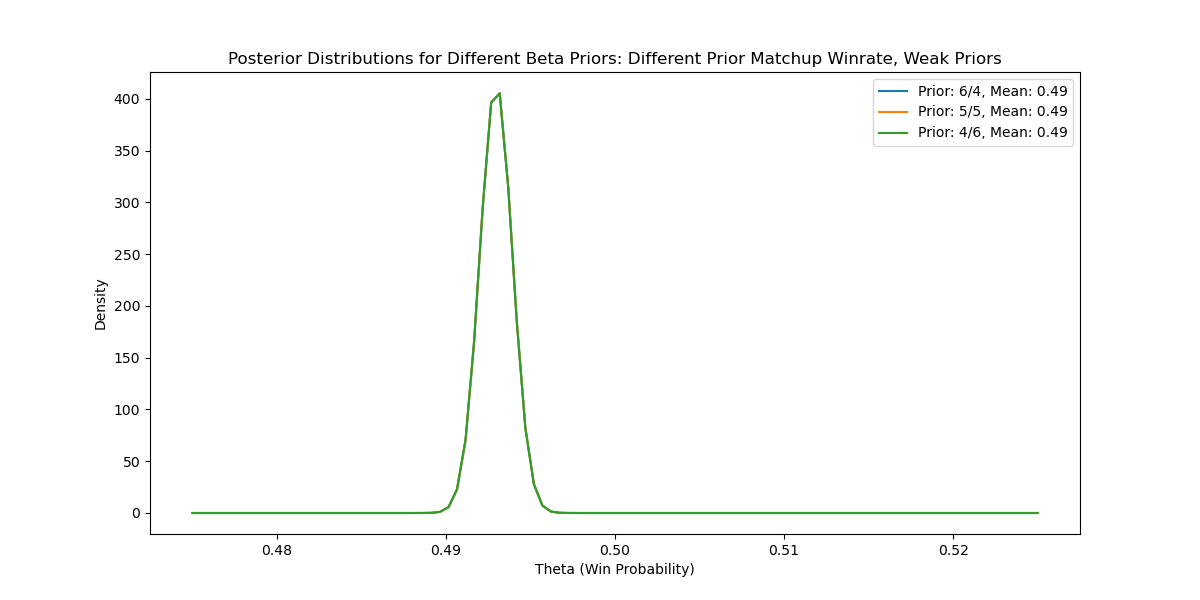
\includegraphics[width=0.8\textwidth]{figures/posterior_beta_priors_varying_matchup_winrate.png}
\caption[Modeling a different Marth-Fox expected win rates with weak priors.]{Modeling a different Marth-Fox expected win rates with weak priors.}
\label{fig:posterior_beta_priors_varying_matchup_winrate}
\end{figure}
\begin{figure}[H]
\center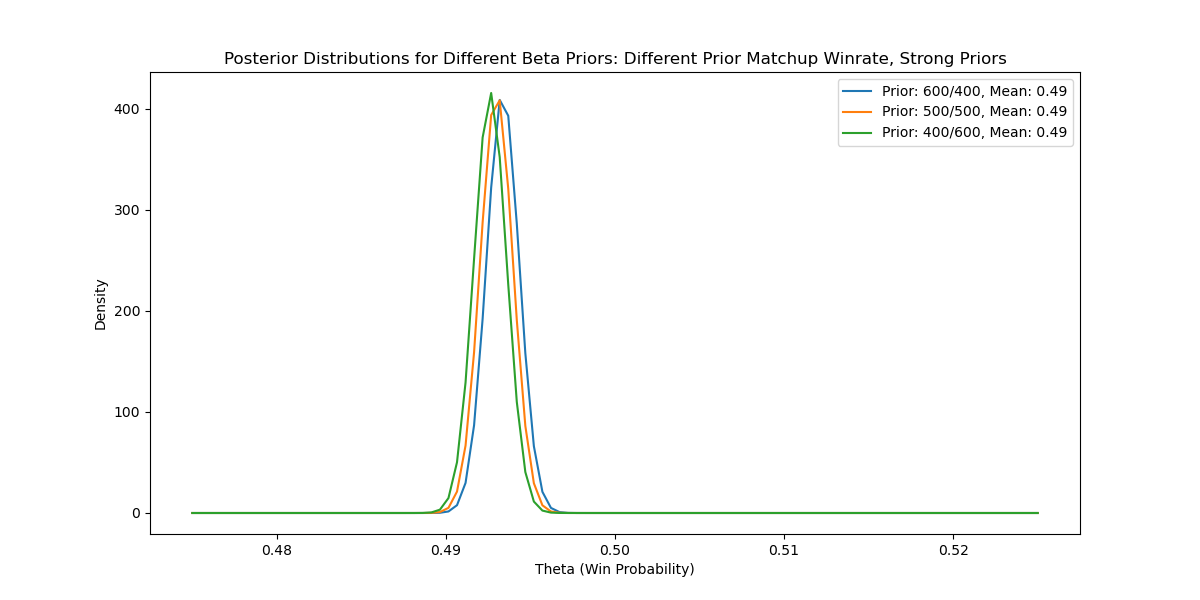
\includegraphics[width=0.8\textwidth]{figures/posterior_beta_priors_varying_matchup_winrate_and_strength.png}
\caption[Modeling a different Marth-Fox expected win rates with strong priors.]{Modeling a different Marth-Fox expected win rates with strong priors.}
\label{fig:posterior_beta_priors_varying_matchup_winrate_and_strength}
\end{figure}
\indent As can be seen in these graphs, the expected win rate of Marth against Fox is greatly impacted by the observed. This makes sense because the posterior distribution parameters will be greatly influenced by the likelihood. Thus, in the case of a large data sample like this, the impact of the priors, regardless of perceived strength, is rendered nearly meaningless due to the sheer amount of observed data there is. However, for cases of uncommon matchups, where there may not be a lot of available data, the Bayesian model will allow our prior to be incorporated into the posterior to a greater degree. Below are graphs of the posterior when in a hypothetical sample of 10 Marth-Fox matches, Marth wins 8 of them.
\begin{figure}[H]
\center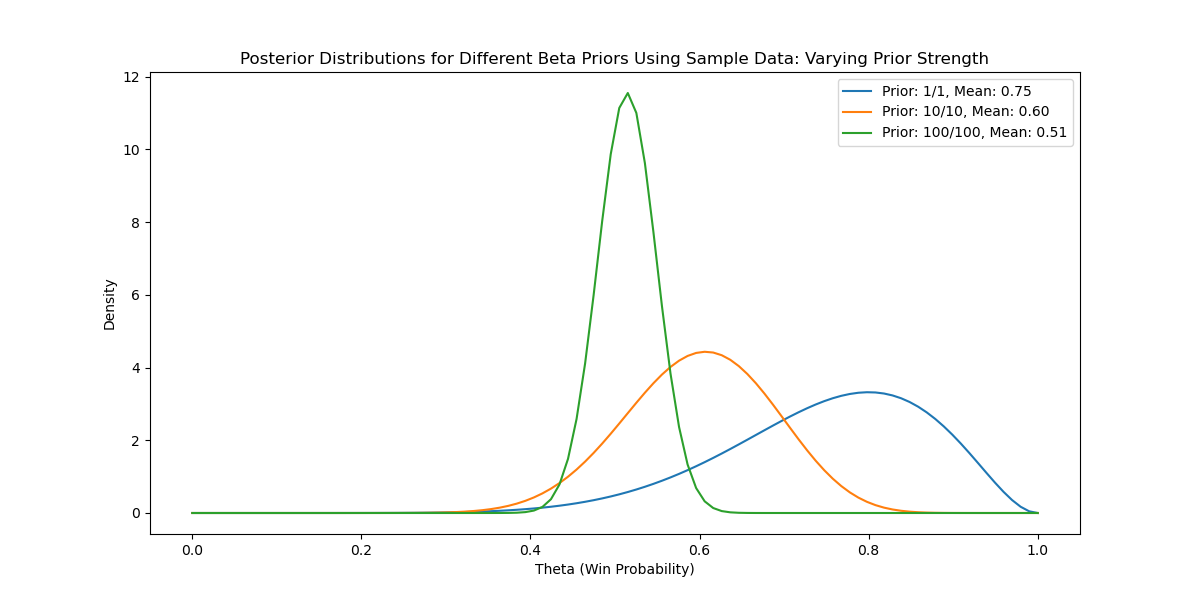
\includegraphics[width=0.8\textwidth]{figures/posterior_beta_priors_sample_data.png}
\caption[Modeling a different Marth-Fox expected win rates given an even (50/50) matchup prior using sample data.]{Modeling a different Marth-Fox expected win rates given an even (50/50) matchup prior using sample data.}
\label{fig:posterior_beta_priors_sample_data}
\end{figure}
\begin{figure}[H]
\center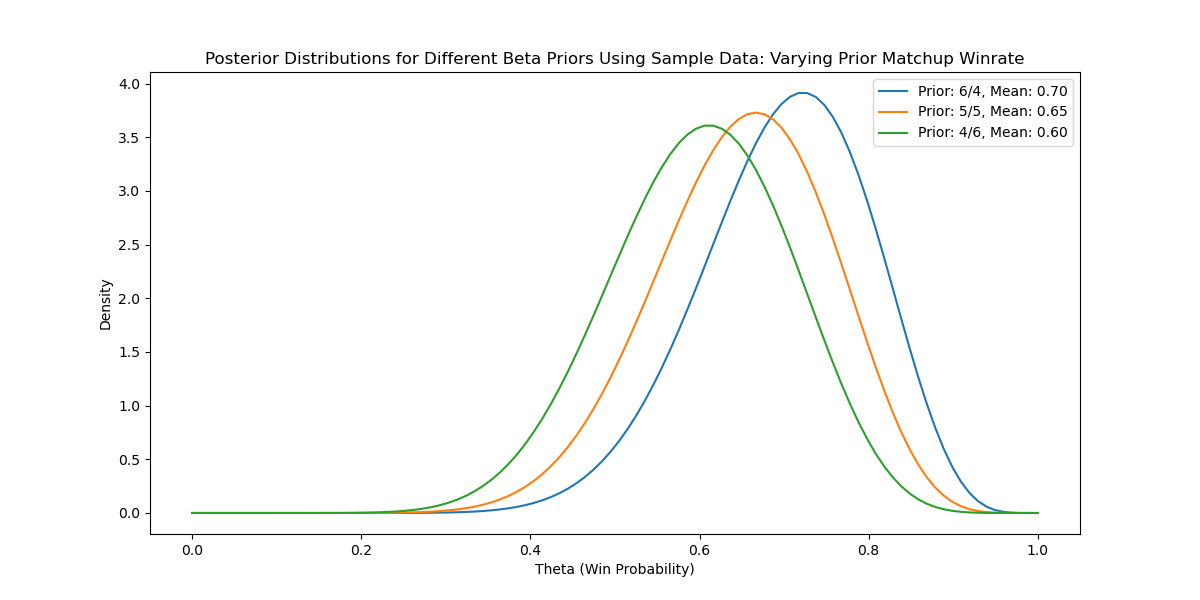
\includegraphics[width=0.8\textwidth]{figures/posterior_different_beta_priors_sample_data.png}
\caption[Modeling a different Marth-Fox expected win rates given varying matchup priors of similar strength using sample data.]{Modeling a different Marth-Fox expected win rates given varying matchup priors of similar stregth using sample data.}
\label{fig:posterior_different_beta_priors_sample_data}
\end{figure}
\indent Looking at the above figures, it is more evident how changing a prior's strength or shape will affect the posterior distribution. Again, in the case of Melee, given $n=26$ characters, there are $\frac{n(n+1)}{2}=\frac{26\cdot27}{2}=351$ total unique matchups. By leveraging a Bayesian approach, we can more accurately model matchup probabilities for characters with significantly lower use rate in competitive settings.

\indent Although this is a good exercise and a simple way to use Bayesian methods to better model matchups in Melee, there are several components not included in this initial model. First, as previously explained, stages in Melee often make a difference in a matchup. In the Marth-Fox matchup, it is argued that Final Destination is a strong choice for Marth due to him gaining access to techniques not available on stages with platforms. Thus, we are interested in also understanding character matchups by stage. Second, it is likely that not all of the observed matches were against evenly matched players. We may want to design a model that factors in player skill when trying to determine the true matchup spread.

\section{Model 2: Marth-Fox Matchup by Stage}
In competitive Melee, there are 6 tournament-legal stages. These are Battlefield, Final Destination, Dream Land, Fountain of Dreams, Pokemon Stadium, and Yoshi's Story. We are interested in understanding how the Marth-Fox matchup varies by stage. In competitive Melee, players will go through a process known as ``stage striking'', in which players take turns removing a stage from being selected until there is only one remaining \citep{SmashWiki_StageStriking}. It is important for a player to understand how their character performs on each stage in a given matchup.

\indent To determine if there is a significant effect a stage has on the Marth-Fox matchup, we can utilize a logistic regression model. This fits since the response data (a match win or loss) is binary in nature. We define our model in the following way:
\begin{align*}
    y_i|p_i\sim\text{Bernoulli}(p_i), i=1,\dots,6\\
    \text{logit}(p_i) = \alpha+\gamma_i\\
    \alpha\sim N(0, 10)\\
    \gamma_i\sim N(0, 10)\\
    \sum\gamma_i = 0
\end{align*}
Where $\alpha$ represents the base ``matchup effect'' and $\gamma_i$ represents the ``stage effect'' on the matchup probability.

\section{Model 3: Factoring in Elo}
In newer versions of Slippi, a ranked mode was added. In this mode, players are given a rating. A higher number is indicative of a more skilled player, and vice versa. We can use this information as a factor in modeling the matchups in Melee.
